\documentclass[border=5pt]{standalone}
\usepackage{amssymb}
\usepackage{tikz}
\usepackage{tikz-inet}
\usepackage{xcolor}

\colorlet{darkred}{red!60!black}
\colorlet{darkblue}{blue!60!black}
\colorlet{darkgreen}{green!60!black}

\usetikzlibrary{positioning, arrows.meta, patterns, calc}
\begin{document}
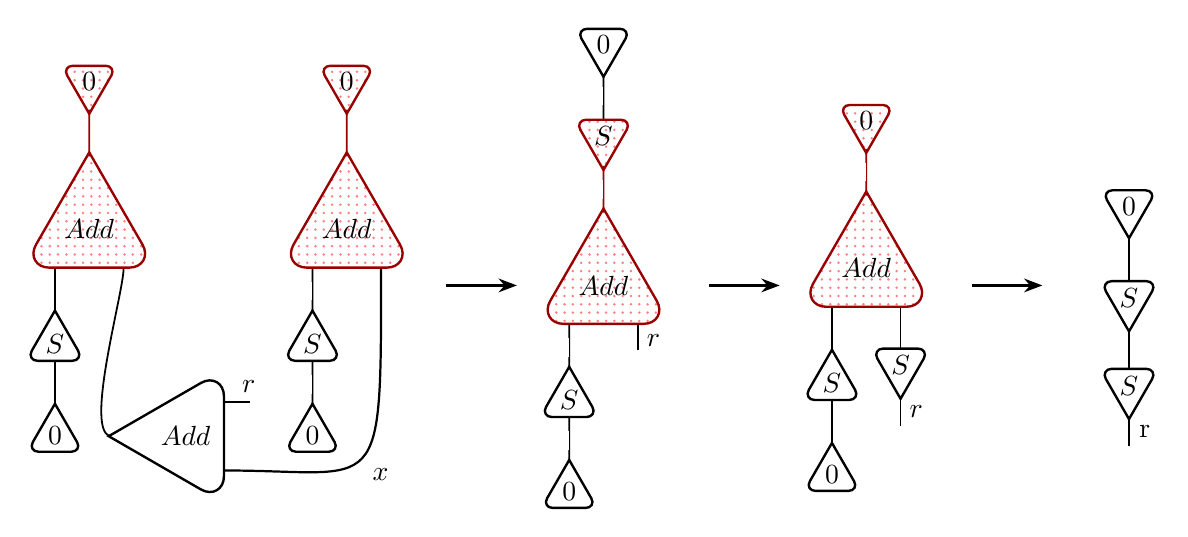
\begin{tikzpicture}[>=Stealth, node distance=0.5cm]

\begin{scope}[local bounding box=group1, baseline=(group1.center)]
    \inetcell[draw=darkred,pattern color=red!50, pattern=dots](add1){$Add$}[U]
    \inetcell[above=of add1.pal, draw=darkred, pattern color=red!50, pattern=dots](zero1){$0$}[D]
    \inetcell[below=of add1.left pax](s1){$S$}[U]
    \inetcell[below=of s1.middle pax](zero2){$0$}[U]
    
    \inetwire[darkred](add1.pal)(zero1.pal)
    \inetwire(add1.left pax)(s1.pal)
    \path (add1.left pax) -- node[left, fill=white] {} (s1.pal);
    \inetwire(s1.middle pax)(zero2.pal)
    \path (s1.middle pax) -- node[left, fill=white] {} (zero2.pal);
    
    \inetcell[below right=5em and 1em of add1](addMain){$Add$}[L]
    \inetwire(add1.right pax)(addMain.pal)
    \path (add1.right pax) -- node[right, fill=white] {} (addMain.pal);
    \inetwirefree(addMain.right pax)
    \node at ($(addMain.right pax) + (0.3, 0.2)$) {$r$};
    
    \inetcell[right=6em of add1, draw=darkred, pattern color=red!50, pattern=dots](add2){$Add$}[U]
    \inetcell[above=of add2.pal, draw=darkred, pattern color=red!50, pattern=dots](zero3){$0$}[D]
    \inetcell[below=of add2.left pax](s2){$S$}[U]
    \inetcell[below=of s2.middle pax](zero4){$0$}[U]
    
    \inetwire[darkred](add2.pal)(zero3.pal)
    \inetwire(add2.left pax)(s2.pal)
    \path (add2.left pax) -- node[left, fill=white] {} (s2.pal);
    \inetwire(s2.middle pax)(zero4.pal)
    \path (s2.middle pax) -- node[left, fill=white] {} (zero4.pal);
    
    \draw[thick] (add2.right pax) .. controls +(down:30mm) and +(right:20mm) .. (addMain.left pax) node[midway, below right, fill=white] {$x$};
\end{scope}

\begin{scope}[shift={(group1.east)}, xshift=2.5cm, local bounding box=group2, baseline=(group2.center)]
    \inetcell[draw=darkred, pattern color=red!50, pattern=dots](addRed1){$Add$}[U]
    \inetcell[above=of addRed1.pal, draw=darkred, pattern color=red!50, pattern=dots](sRed1){$S$}[D]
    \inetcell[above = of sRed1.middle pax](zeroRed1){$0$}[D]
    \inetcell[below= of addRed1.left pax](sRed2){$S$}[U]
    \inetcell[below= of sRed2.middle pax](zeroRed2){$0$}[U]
    
    \inetwire(zeroRed1.pal)(sRed1.middle pax)
    \path (zeroRed1.pal)-- node[left, fill=white] {} (sRed1.middle pax);
    \inetwire(zeroRed2.pal)(sRed2.middle pax)
    \path (zeroRed2.pal) -- node[left, fill=white] {} (sRed2.middle pax);
    \inetwire(sRed2.pal)(addRed1.left pax)
    \path (sRed2.pal) -- node[left, fill=white] {} (addRed1.left pax);
    \inetwire[darkred](sRed1.pal)(addRed1.pal)
    \path (sRed1.pal) -- node[left, fill=white] {} (addRed1.pal);
    \inetwirefree(addRed1.right pax)
    \node at ($(addRed1.right pax) + (0.2, -0.2)$) {$r$};
\end{scope}


\begin{scope}[shift={(group2.east)}, xshift=2.5cm, local bounding box=group3, baseline=(group3.center)]
    \inetcell[draw=darkred, pattern color=red!50, pattern=dots](addRed1){$Add$}[U]
    \inetcell[below=of addRed1.right pax](sRed1){$S$}[D]
    \inetcell[above=of addRed1.pal, draw=darkred, pattern color=red!50, pattern=dots](zeroRed1){$0$}[D]
    \inetcell[below= of addRed1.left pax](sRed2){$S$}[U]
    \inetcell[below= of sRed2.middle pax](zeroRed2){$0$}[U]
    
    \inetwire[darkred](zeroRed1.pal)(addRed1.pal)
    \path (zeroRed1.pal) -- node[left, fill=white] {} (addRed1.pal);
    \inetwire(zeroRed2.pal)(sRed2.middle pax)
    \path (zeroRed2.pal) -- node[left, fill=white] {}(sRed2.middle pax);
    \inetwire(sRed2.pal)(addRed1.left pax)
    \path (sRed2.pal) -- node[left, fill=white] {} (addRed1.left pax);
    \inetwire(sRed1.middle pax)(addRed1.right pax)
    \path (sRed1.middle pax) -- node[right, fill=white] {}(addRed1.right pax);
    \inetwirefree(sRed1.pal)
    \node at ($(sRed1.pal) + (0.2, -0.2)$) {$r$};
\end{scope}

\begin{scope}[shift={(group3.east)}, xshift=2.5cm]
    \inetcell(sRed1){$S$}[D]
    \inetcell[above = of sRed1.middle pax](zeroRed1){$0$}[D]
    \inetcell[below = of sRed1.pal](sRed2){$S$}[D]
    
    \inetwire(zeroRed1.pal)(sRed1.middle pax)
    \path (zeroRed1.pal)-- node[right, fill=white] {} (sRed1.middle pax);
    \inetwire(sRed1.pal)(sRed2.middle pax)
    \path (sRed1.pal) -- node[right, fill=white] {}(sRed2.middle pax);
    \inetwirefree(sRed2.pal)
    \node at ($(sRed2.pal) + (0.2, -0.2)$) {r};
\end{scope}


\coordinate (arrowY) at (group1.east);

\draw[->, thick] ([xshift=0.5cm]group1.east) -- ++(0.9,0);
\draw[->, thick] ([xshift=0.5cm]group2.east |- arrowY) -- ++(0.9,0);
\draw[->, thick] ([xshift=0.5cm]group3.east |- arrowY) -- ++(0.9,0);

\end{tikzpicture}
\end{document}
